\documentclass[margin,line]{resume}

\definecolor{sidebarcolor}{RGB}{73, 19, 92}

\usepackage[utf8]{inputenc}
\usepackage[T2A]{fontenc}
\usepackage[english,russian]{babel}
\usepackage{fontawesome}

\newcommand{\githubrepos}{73}
\newcommand{\githubcommits}{1597}
\newcommand{\githublines}{297996}

\begin{document}

{\vspace*{-13mm}\sc \large Гришин Антон — DevOps инженер} \\
\begin{resume}
  \begin{minipage}[t]{0.55\textwidth}
    \section{\mysidestyle Персональная\\Информация}
    Москва, Россия \\
    \faAlcehmmist\space
    \href{https://alchemmist.xyz}{\texttt{alchemmist.xyz}} \\
    \faGithub  \space
    \href{https://github.com/alchemmist/}{\texttt{alchemmist}} \\
    \faLinkedin \space
    \href{https://www.linkedin.com/in/alchemmist/}{\texttt{alchemmist}}
    \\
    \faPaperPlane \space \href{https://t.me/alchemmist}{\texttt{@alchemmist}} \\
    \faPhone \space
    \href{tel:+79150672638}{\color{linkcolor}\texttt{+7(915)067-2638}}  \\
    \faEnvelope \space
    \href{mailto:anton.ingrish@gmail.com}{\color{linkcolor}\texttt{anton.ingrish@gmail.com}}
  \end{minipage}

  \begin{minipage}[H]{0.18\textwidth}
    \begin{textblock}{7}(10.87, 1.38)
      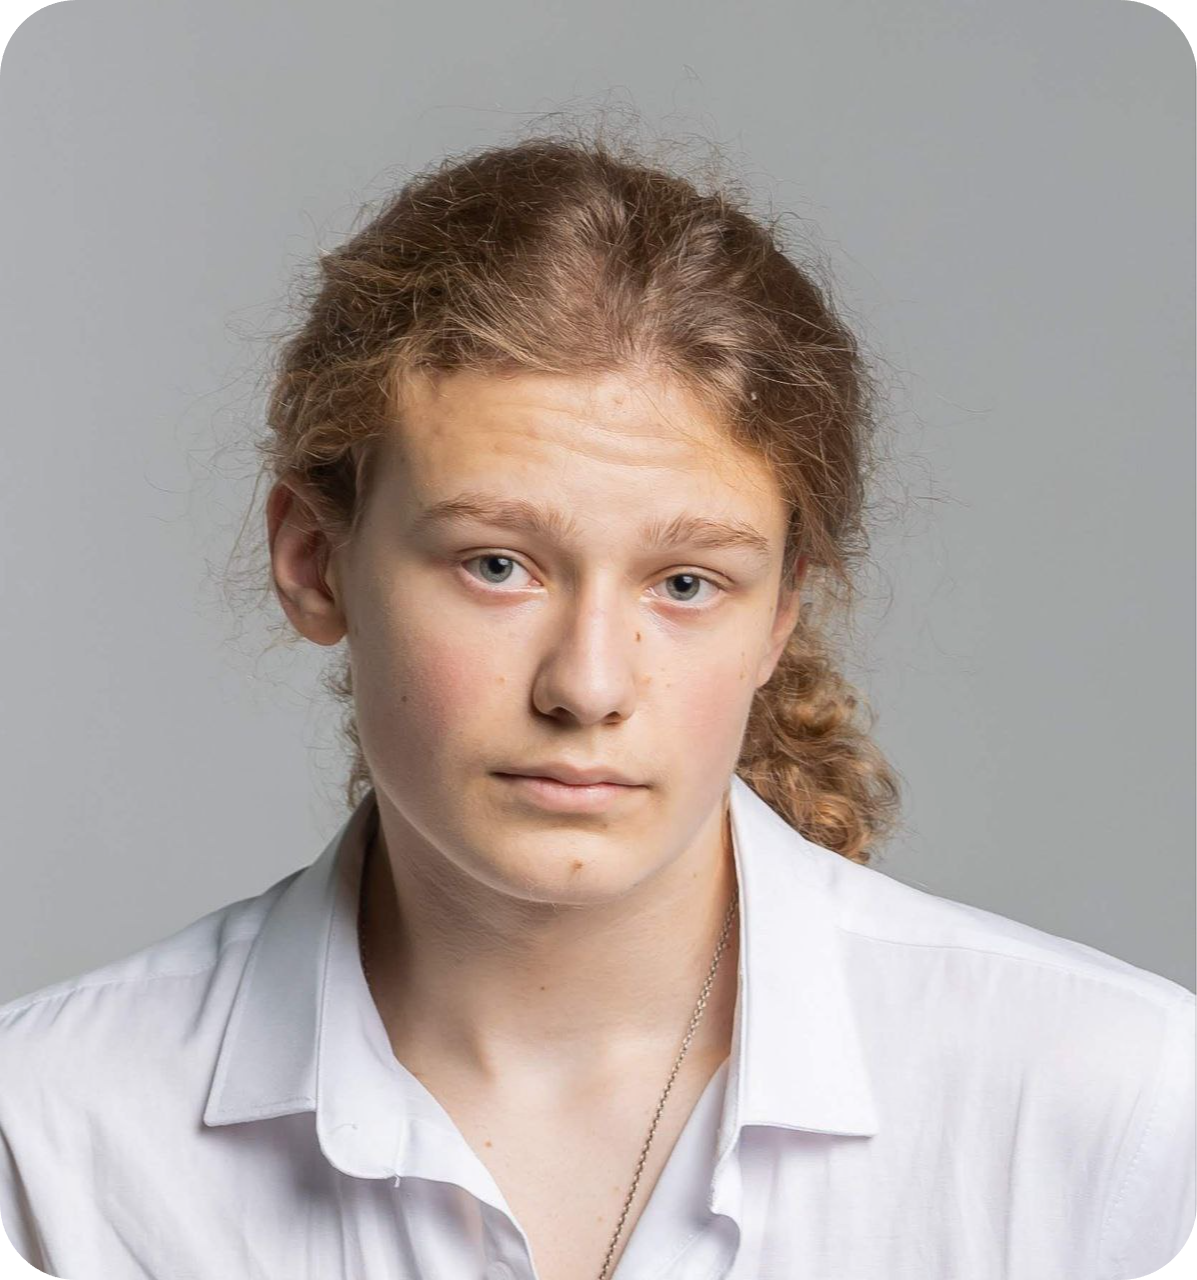
\includegraphics[width=0.270\textwidth]{../images/avatar.png}
    \end{textblock}
  \end{minipage}

  \vspace{-8mm}
  \section{\mysidestyleОбо мне}
  Инженер с фокусом на инфраструктуру и автоматизацию разработки.
  Проектирую воспроизводимые окружения, настраиваю CI/CD пайплайны
  и разрабатываю инструменты для разработчиков.

  Глубоко работаю с Linux: конфигурация системы, автоматизация,
  CLI-инструменты и оптимизация developer workflow.
  Имею опыт построения сервисной архитектуры и подготовки сервисов к деплою.

  \vspace{-1mm}

  \section{\mysidestyleОбразование}
  \href{https://cu.ru/}{Центральный Университет},
  Математика и компьютерные науки, трек «Разработка», 2028.

  \href{https://lyceum.yandex.ru/}{Лицей
  Академии Яндекса}, направление «Промышленная Разработка», 2023.
  (\href{https://alchemmist.github.io/CV/attachments/yandex-lyceum.pdf}{диплом})

  Курс
  \texttt{\href{https://softwarefoundations.cis.upenn.edu}{softwarefoundations}}.
  Прочитал первый том,
  \href{https://github.com/alchemmist/coq-learning}{доказал} 250
  теорем на \inlinecode{Coq}.

  \vspace{-1mm}

  \section{\mysidestyleПроекты}\vspace{0mm}
  \begin{description}[leftmargin=0pt, itemindent=*, itemsep=8pt]

    \item[Devsyringe:]
      \href{https://devsyringe.alchemmist.xyz/}{CLI-инструмент}
      для управления конфигурацией через декларативные YAML-правила.
      Реализовал TUI-интерфейс и систему команд.

      Настроил CI/CD пайплайны сборки и релизов (GitHub Actions),
      автоматическую публикацию и кроссплатформенную дистрибуцию
      через \texttt{Go}, \texttt{AUR} и \texttt{brew}.

      Стек: \inlinecode{Go}, \inlinecode{bubbletea},
      \inlinecode{cobra}, \inlinecode{CI/CD}, \inlinecode{Linux}.

    \item[lazy-tmux:]
      \href{https://lazy-tmux.xyz}{CLI-инструмент}
      для управления окружениями разработчика.

      Реализовал сериализацию и восстановление tmux-сессий,
      что позволяет воспроизводить рабочее окружение.
      Добавил автоматизацию конфигурации и навигации между сессиями.

      Стек: \inlinecode{Go}, \inlinecode{tmux}, \inlinecode{Linux}.

    \item[Ballkit:]
      \href{https://github.com/ballkit}{Система лояльности}.
      Спроектировал backend-сервис и взаимодействие через gRPC.

      Подготовил проект к деплою: настроил окружение,
      структуру сервиса и процесс сборки.

      Стек: \inlinecode{Go}, \inlinecode{grpc}, \inlinecode{Docker}.

    \item[SmartCab:]
      \href{https://github.com/smart-cab}{IoT-система умного дома}.

      Настроил взаимодействие устройств через MQTT брокер,
      реализовал backend и инфраструктуру обмена данными между сервисами.

      Стек: \inlinecode{Python}, \inlinecode{Go},
      \inlinecode{Mosquitto}, \inlinecode{redis}, \inlinecode{postgres}.

  \end{description}

  \section{\mysidestyleДостижения}
  Финалист
  (\href{https://alchemmist.github.io/CV/attachments/russian-chemp-final.pdf}{\texttt{1}})
  \href{https://events.fsp-russia.com/championship}{Чемпионата
  России} по спортивному программированию.

  Разработал микросервисную архитектуру из 9 сервисов,
  настроил взаимодействие через брокеры сообщений и API.

  Стек:
  \inlinecode{Kafka}, \inlinecode{RabbitMQ}, \inlinecode{FastAPI}.

  \href{https://alchemmist.github.io/CV/attachments/scince-for-life-win.pdf}{Победитель}
  конференции «Наука для жизни» с IoT-проектом.
  Реализовал инфраструктуру обмена данными между устройствами.

  \section{\mysidestyleНавыки}
  \inlinecode{Linux}, \inlinecode{bash}, \inlinecode{tmux},
  \inlinecode{Docker}, \inlinecode{Podman},
  \inlinecode{CI/CD (GitHub Actions)},
  \inlinecode{Git}, \inlinecode{Make},
  \inlinecode{RabbitMQ}, \inlinecode{Mosquitto},
  \inlinecode{postgres}, \inlinecode{redis},
  \inlinecode{Go}, \inlinecode{Python},
  \inlinecode{grpc}, \inlinecode{HTTP APIs}.

\end{resume}

\clearpage

\end{document}
